\documentclass[conference]{IEEEtran}
\IEEEoverridecommandlockouts
\usepackage{cite}
\usepackage{amsmath,amssymb,amsfonts}
\usepackage{graphicx}
\usepackage{booktabs}
\usepackage{multirow}
\usepackage{xcolor}
\usepackage{url}
\usepackage{tikz}
\usetikzlibrary{positioning,arrows.meta,fit,backgrounds,calc}
\usepackage[hidelinks]{hyperref}

\newcommand{\RTS}{\mathrm{RTS}}
\newcommand{\best}[1]{\textbf{#1}}

\begin{document}

% =====================================================================
% 1. TITLE
% =====================================================================
\title{Hallucination-Aware Hybrid RAG with a Retrieval Transparency Score (RTS~v2) for Scientific Claim Verification}

\author{
\IEEEauthorblockN{Prithviraj Jhunjhunwala (2310110232), Diggaj Rupani, Saksham Dhawan, Amey Gautam}
\IEEEauthorblockA{\textit{Department of Computer Science and Engineering}, \textit{Shiv Nadar University}, India\\
CSD358 Information Retrieval --- Final Project (extension of the mid-term project, Track T1)}
}

\maketitle

% =====================================================================
% 2. ABSTRACT
% =====================================================================
\begin{abstract}
Retrieval-augmented generation (RAG) systems can produce fluent answers that the retrieved sources do not support, which
is unacceptable in science and medicine. We present a hallucination-aware hybrid RAG pipeline for scientific claim
verification on BEIR SciFact that (i) retrieves evidence with a hybrid of from-scratch lexical models (TF-IDF, BM25,
query likelihood, RM3) and dense encoders fused by weighted Reciprocal Rank Fusion and re-ranked by a cross-encoder;
(ii) generates a verdict with sentence-level citations using a local 3B-parameter LLM; and (iii) verifies every generated
sentence with the \emph{Retrieval Transparency Score v2} (RTS~v2), which combines span-level attribution, semantic
similarity and natural language inference (NLI) with an explicit contradiction penalty and a citation-faithfulness check.
All parameters are tuned on the SciFact train split only. Retrieval reaches NDCG@10 $=0.766$ ($+0.078$ over our mid-term
system, $p<0.001$), above every SciFact system reported in the BEIR paper, and transfers without re-tuning to NFCorpus and
FiQA. On a 677-sentence test benchmark, RTS~v2 detects hallucinated sentences with ROC-AUC $0.958$ (mid-term RTS~v1:
$0.660$) and catches 95.6\% of negations versus 75.6\%. RTS-guided verification raises claim-level macro-F1 from $0.414$
(LLM alone, which never outputs \emph{refuted}) to $0.673$, and abstract-level label-only F1 to $56.6$ versus $51.0$ for
the VeriSci baseline of the SciFact paper. A human evaluation on 80 real LLM sentences shows a large gap between benchmark
and real-world detection (ROC-AUC $0.573$), which we analyse as the main limitation.
\end{abstract}

\begin{IEEEkeywords}
retrieval-augmented generation, hybrid retrieval, reciprocal rank fusion, hallucination detection, natural language
inference, scientific claim verification, BEIR, SciFact
\end{IEEEkeywords}

% =====================================================================
% 3. INTRODUCTION
% =====================================================================
\section{Introduction}
\textbf{Background.} Retrieval-augmented generation grounds a language model in documents retrieved from a corpus
\cite{lewis2020rag}. Two components decide its quality: the \emph{retriever}, which must surface the right evidence, and
the \emph{generator}, which must say only what that evidence supports. Large language models (LLMs) are known to produce
fluent but unsupported or contradictory content, commonly called hallucination \cite{ji2023survey}.

\textbf{Importance and motivation.} In scientific and biomedical settings a confident but wrong statement, such as
reversing the direction of a treatment effect, can mislead readers more than no answer at all. A trustworthy system
should therefore (a) find the right evidence, (b) cite it, and (c) tell the user, sentence by sentence, how far each
statement is backed by the evidence. Our mid-term system built a hybrid retriever and a first transparency score
(RTS~v1) based only on cosine similarity. Error analysis showed that cosine similarity cannot see negation (``X
\emph{increases} Y'' and ``X \emph{decreases} Y'' have nearly identical embeddings), that scoring extractive sentences
against the documents they were copied from is close to circular, and that the dense encoder truncated documents to 256
characters.

\textbf{Contributions.} This final project substantially extends the mid-term work:
\begin{enumerate}
\item A reproducible, \texttt{trec\_eval}-verified hybrid retrieval pipeline (inverted index, TF-IDF, BM25, query
likelihood, RM3 and RRF implemented from scratch, plus dense retrieval and cross-encoder re-ranking), tuned on the train
split only. It reaches NDCG@10 $=0.766$ on SciFact and generalises zero-shot to NFCorpus and FiQA.
\item Generative claim verification with sentence-level citations using a local LLM, with an analysis showing that the
generator's reasoning, not retrieval, is the bottleneck.
\item \textbf{RTS~v2}, a sentence-level transparency score that combines span attribution, similarity and NLI with a
contradiction penalty, and reports provenance and citation faithfulness for every sentence.
\item RTS-guided verdict correction that fixes the LLM's inability to refute claims, compared with the SciFact paper
\cite{wadden2020scifact} and the BEIR paper \cite{thakur2021beir}.
\item An honest evaluation that includes significance tests, ablations, generalisation, a human evaluation on real LLM
outputs and two negative results.
\end{enumerate}
Table~\ref{tab:midterm} summarises what was added after the mid-term.

\begin{table}[t]
\centering
\caption{Mid-term system vs.\ final project}
\label{tab:midterm}
\footnotesize
\begin{tabular}{@{}p{0.27\columnwidth}p{0.29\columnwidth}p{0.34\columnwidth}@{}}
\toprule
Component & Mid-term & Final project \\
\midrule
Lexical retrieval & Zone TF-IDF (labelled lnc.ltc, ran ltc.ltc), BM25 & Corrected lnc.ltc, from-scratch BM25, QL-Dirichlet, RM3; all tuned on train \\
Dense retrieval & MiniLM, 256 characters & Full abstracts; BGE-base \\
Fusion / ranking & RRF of top-20, equal weights & Weighted deep RRF (subset + weights + $k$ tuned); cross-encoder re-ranking \\
Generation & Extractive sentences & Qwen2.5-3B verdict with sentence-level citations \\
Verification & RTS v1: cosine to first 400 chars & RTS v2: spans + similarity + NLI + contradiction penalty + citation check; verdict correction \\
Evaluation & MAP@10, MRR, NDCG@10; 50-query RTS ablation & 10 retrieval metrics (\texttt{trec\_eval}-verified), significance tests, P/R/F1/Accuracy for detection and verification, human labels, 2 paper comparisons, 2 extra datasets \\
Demo & Notebook & Live Gradio app with hallucination injection \\
\bottomrule
\end{tabular}
\end{table}

% =====================================================================
% 4. RELATED WORK
% =====================================================================
\section{Literature Review / Related Work}
\textbf{Lexical retrieval.} The vector space model with SMART weighting (e.g.\ lnc.ltc) \cite{manning2008ir} and the
probabilistic BM25 model \cite{robertson2009bm25} remain strong baselines. Language-model retrieval scores documents by
query likelihood with Dirichlet smoothing \cite{zhai2001smoothing}, and relevance models (RM3) expand queries with terms
from pseudo-relevant documents \cite{lavrenko2001relevance}.

\textbf{Dense retrieval, fusion and re-ranking.} Sentence-BERT \cite{reimers2019sbert} and later embedding models such as
BGE \cite{xiao2024cpack} encode queries and documents into a shared vector space searched with FAISS \cite{johnson2021faiss}.
Reciprocal Rank Fusion combines rankings without score calibration \cite{cormack2009rrf}, and BERT cross-encoders re-rank
candidates by reading query and passage jointly \cite{nogueira2019passage}. BEIR \cite{thakur2021beir} evaluates such
models zero-shot on 18 datasets, including SciFact, NFCorpus and FiQA, and found BM25 to be a robust baseline.

\textbf{Retrieval-augmented generation and attribution.} RAG \cite{lewis2020rag} conditions generation on retrieved
passages. ALCE \cite{gao2023alce} asks LLMs to cite their sources and measures citation quality with NLI.

\textbf{Scientific fact verification.} FEVER \cite{thorne2018fever} established claim verification against Wikipedia.
SciFact \cite{wadden2020scifact} introduced expert-written scientific claims labelled SUPPORT, CONTRADICT or NEI against
paper abstracts with rationale sentences, and the VeriSci baseline, a pipeline of abstract retrieval, rationale selection
and label prediction.

\textbf{Hallucination detection.} Surveys catalogue hallucination types and detection methods \cite{ji2023survey}.
NLI-based consistency checking is among the strongest approaches \cite{honovich2022true, laban2022summac}, using models
such as DeBERTa \cite{he2023debertav3}. SelfCheckGPT detects hallucinations from sampling inconsistency without
retrieval \cite{manakul2023selfcheckgpt}, and FActScore decomposes generations into atomic facts \cite{min2023factscore}.

\textbf{Novelty of our approach.} Prior work typically uses either similarity-based attribution or NLI-based consistency,
evaluates retrieval and generation separately, and rarely reports results on real generated text. We (i) integrate
from-scratch IR models, dense retrieval, tuned fusion and re-ranking with sentence-level verification in one pipeline;
(ii) define RTS~v2, which unifies span provenance, similarity, entailment, an explicit contradiction penalty and citation
faithfulness into one interpretable per-sentence score with calibrated labels; (iii) use the claim-level evidence check to
correct the generator's verdicts; and (iv) validate against human SciFact labels, controlled perturbations and our own
labels of real LLM sentences, under a strict train/test protocol.

% =====================================================================
% 5. OBJECTIVE
% =====================================================================
\section{Objective}
\begin{enumerate}
\item[O1] Significantly improve evidence retrieval over the mid-term system, using only train data for model selection.
\item[O2] Generate verdicts with sentence-level citations from the retrieved evidence.
\item[O3] Design a sentence-level transparency score that detects unsupported and contradicted statements and explains
its decision with evidence.
\item[O4] Use the verification signal to improve the verdicts themselves.
\item[O5] Evaluate rigorously: standard metrics, significance tests, ablations, comparison with published work,
generalisation and human judgement.
\end{enumerate}

% =====================================================================
% 6. PROPOSED MODEL
% =====================================================================
\section{Proposed Model}
\begin{figure*}[t]
\centering
\resizebox{\textwidth}{!}{%
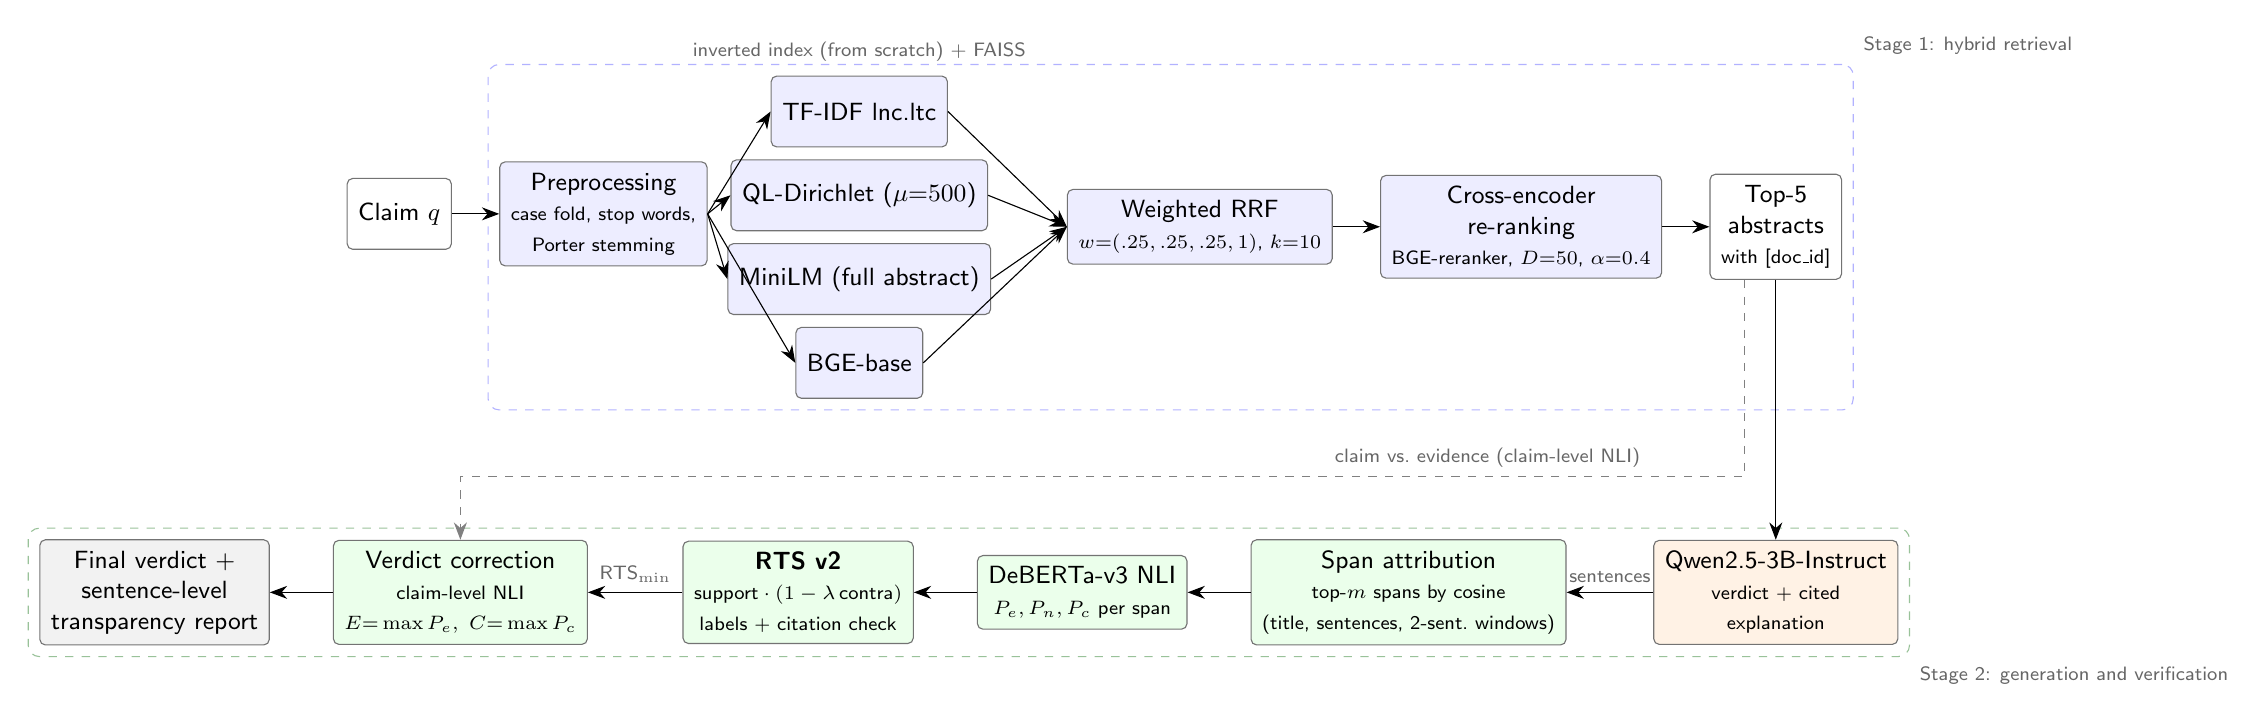
\begin{tikzpicture}[
  font=\sffamily\small, >={Stealth[length=2.2mm]},
  box/.style={draw=black!55, rounded corners=2pt, align=center, inner sep=4pt, minimum height=9mm, fill=white},
  ir/.style={box, fill=blue!7}, gen/.style={box, fill=orange!10}, ver/.style={box, fill=green!8},
  lab/.style={font=\sffamily\scriptsize, text=black!60}]
% ---- row 1: retrieval
\node[box] (claim) {Claim $q$};
\node[ir, right=6mm of claim] (pre) {Preprocessing\\{\scriptsize case fold, stop words,}\\{\scriptsize Porter stemming}};
\node[ir, right=8mm of pre, yshift=13mm] (tfidf) {TF-IDF lnc.ltc};
\node[ir, below=1.5mm of tfidf] (ql) {QL-Dirichlet ($\mu{=}500$)};
\node[ir, below=1.5mm of ql] (mini) {MiniLM (full abstract)};
\node[ir, below=1.5mm of mini] (bge) {BGE-base};
\node[lab, above=0.5mm of tfidf] {inverted index (from scratch) + FAISS};
\node[ir, right=10mm of ql, yshift=-4mm] (rrf) {Weighted RRF\\{\scriptsize $w{=}(.25,.25,.25,1)$, $k{=}10$}};
\node[ir, right=6mm of rrf] (ce) {Cross-encoder\\re-ranking\\{\scriptsize BGE-reranker, $D{=}50$, $\alpha{=}0.4$}};
\node[box, right=6mm of ce] (top) {Top-5\\abstracts\\{\scriptsize with [doc\_id]}};
% ---- row 2: generation + verification
\node[gen, below=33mm of top] (llm) {Qwen2.5-3B-Instruct\\{\scriptsize verdict + cited}\\{\scriptsize explanation}};
\node[ver, left=11mm of llm] (span) {Span attribution\\{\scriptsize top-$m$ spans by cosine}\\{\scriptsize (title, sentences, 2-sent.\ windows)}};
\node[ver, left=8mm of span] (nli) {DeBERTa-v3 NLI\\{\scriptsize $P_e, P_n, P_c$ per span}};
\node[ver, left=8mm of nli] (rts) {\textbf{RTS v2}\\{\scriptsize $\text{support}\cdot(1-\lambda\,\text{contra})$}\\{\scriptsize labels + citation check}};
\node[ver, left=12mm of rts] (verd) {Verdict correction\\{\scriptsize claim-level NLI}\\{\scriptsize $E{=}\max P_e,\ C{=}\max P_c$}};
\node[box, left=8mm of verd, fill=black!5] (out) {Final verdict +\\sentence-level\\transparency report};
% ---- arrows
\draw[->] (claim) -- (pre);
\foreach \n in {tfidf,ql,mini,bge} {\draw[->] (pre.east) -- (\n.west); \draw[->] (\n.east) -- (rrf.west);}
\draw[->] (rrf) -- (ce); \draw[->] (ce) -- (top); \draw[->] (top) -- (llm);
\draw[->] (llm) -- node[lab, above] {sentences} (span);
\draw[->] (span) -- (nli); \draw[->] (nli) -- (rts); \draw[->] (rts) -- node[lab, above] {RTS$_{\min}$} (verd); \draw[->] (verd) -- (out);
\draw[->, dashed, black!50] ([xshift=-4mm]top.south) |- ([yshift=8mm]verd.north) node[lab, above, pos=0.6] {claim vs.\ evidence (claim-level NLI)} -- (verd.north);
\begin{scope}[on background layer]
\node[fit=(pre)(tfidf)(bge)(rrf)(ce)(top), draw=blue!30, dashed, rounded corners, inner sep=4pt,
      label={[lab]north east:Stage 1: hybrid retrieval}] {};
\node[fit=(out)(verd)(rts)(nli)(span)(llm), draw=green!40!black!40, dashed, rounded corners, inner sep=4pt,
      label={[lab]south east:Stage 2: generation and verification}] {};
\end{scope}
\end{tikzpicture}}
\caption{Proposed pipeline. Stage~1 retrieves evidence with four retrievers (BM25 and RM3 were also tuned but received
weight 0 in the fusion), fused by weighted RRF and re-ranked. Stage~2 generates a cited verdict, verifies every sentence
with RTS~v2 and corrects the verdict with a claim-level evidence check.}
\label{fig:pipeline}
\end{figure*}

Fig.~\ref{fig:pipeline} shows the pipeline. Given a claim, \textbf{Stage~1} preprocesses it and queries four retrievers:
two lexical models over our own inverted index and two dense encoders over FAISS. Their top-100 lists are fused with
weighted RRF and the top-50 are re-ranked by a cross-encoder. The top-5 abstracts, each tagged with its \texttt{[doc\_id]},
form the evidence. In \textbf{Stage~2}, Qwen2.5-3B-Instruct \cite{qwen2024} writes a verdict (SUPPORTED, REFUTED or NOT
ENOUGH INFO) and a 2--4 sentence explanation in which every sentence cites the abstracts it relies on. Each factual
sentence is attributed to its best evidence spans and checked by an NLI model; RTS~v2 combines both signals into a score,
a label and a citation check. Finally, a claim-level NLI check of the claim against the evidence corrects the LLM verdict.
The output is a verdict plus a sentence-by-sentence transparency report.

% =====================================================================
% 7. METHODOLOGY
% =====================================================================
\section{Methodology}
\subsection{Preprocessing and lexical models}
Text is case-folded, non-alphabetic characters are removed, and tokens are filtered with the NLTK English stop-word list
($|t|>1$) and Porter-stemmed; title and body are indexed as separate zones of one inverted index ($5{,}183$ documents,
$20{,}865$ terms). With $\mathrm{idf}_t=\log(N/\mathrm{df}_t)$ and zone-weighted term frequency
$tf^{z}_{t,d}=w_{T}\,tf^{\text{title}}_{t,d}+w_{B}\,tf^{\text{body}}_{t,d}$, the \textbf{lnc.ltc} model scores
\begin{equation}
s(q,d)=\sum_{t\in q}\frac{(1+\log tf_{t,q})\,\mathrm{idf}_t}{\lVert\mathbf{q}\rVert}\cdot\frac{1+\log tf^{z}_{t,d}}{\lVert\mathbf{d}\rVert},
\end{equation}
i.e.\ log-TF with IDF and cosine normalisation for the query, log-TF without IDF for documents. (The mid-term code
multiplied document weights by IDF, i.e.\ ltc.ltc; we evaluate both.) \textbf{BM25} uses the non-negative Lucene IDF $\mathrm{idf}^{L}_t=\log\big(1+\frac{N-\mathrm{df}_t+0.5}{\mathrm{df}_t+0.5}\big)$:
\begin{equation}
\mathrm{BM25}(q,d)=\sum_{t\in q}\mathrm{idf}^{L}_t\,\frac{tf_{t,d}\,(k_1+1)}{tf_{t,d}+k_1\big(1-b+b\,\frac{|d|}{\mathrm{avgdl}}\big)}.
\end{equation}
\textbf{Query likelihood} with Dirichlet smoothing \cite{zhai2001smoothing}, in rank-equivalent form, with $P(t|C)=cf_t/|C|$:
\begin{equation}
\log P(q|d)\stackrel{rank}{=}\!\sum_{t\in q\cap d}\!c(t,q)\log\!\Big(1+\frac{tf_{t,d}}{\mu P(t|C)}\Big)+|q|\log\frac{\mu}{|d|+\mu}.
\end{equation}
\textbf{RM3} \cite{lavrenko2001relevance} estimates a relevance model from the top-$m$ BM25 documents $F$ with
normalised scores $s(d)$, keeps the top-$n$ terms and interpolates with the original query:
\begin{gather}
P(w|R)\propto\sum_{d\in F}\frac{tf_{w,d}}{|d|}\cdot\frac{s(d)}{\sum_{d'\in F}s(d')},\\
q'(w)=\lambda\,\frac{c(w,q)}{|q|}+(1-\lambda)\,P(w|R).
\end{gather}

\subsection{Dense retrieval, fusion and re-ranking}
Dense scores are cosine similarities of L2-normalised embeddings, $s(q,d)=E(q)^{\top}E(d)$, searched exactly with FAISS
\texttt{IndexFlatIP}. We use MiniLM (\texttt{all-MiniLM-L6-v2}) on \texttt{title.\ abstract} and BGE-base-en-v1.5
\cite{xiao2024cpack} with its query instruction. \textbf{Weighted RRF} \cite{cormack2009rrf} fuses the top-100 of each
retriever $i$:
\begin{equation}
\mathrm{RRF}(d)=\sum_i \frac{w_i}{k+\mathrm{rank}_i(d)}.
\end{equation}
A cross-encoder scores the top-$D$ fused documents, and the final score interpolates per-query min--max normalised scores:
$s(d)=\alpha\,\hat{s}_{CE}(d)+(1-\alpha)\,\hat{s}_{RRF}(d)$.

\subsection{Generation}
The LLM receives a system instruction (``use ONLY the provided abstracts''), the claim and the top-5 abstracts, and must
answer in the format \texttt{VERDICT: \ldots\ EXPLANATION: \ldots}, ending every sentence with \texttt{[doc\_id]}
citations. Decoding is greedy (max.\ 220 new tokens, fp16) for reproducibility. A robust parser maps the verdict to
\{SUPPORT, CONTRADICT, NEI\}, splits sentences, extracts citations and flags citations to abstracts outside the context.

\subsection{Retrieval Transparency Score v2}
For a generated sentence $s$ and context documents $D$: (1) \emph{meta} sentences (abstentions such as ``none of the
abstracts address\ldots'') are detected by rules and not scored; leading attributions (``Abstract X reports that'') are
stripped. (2) Every abstract is split into spans $\mathcal{S}(d)$: title, sentences and all 2-sentence windows; the top-$m$
($m{=}5$) spans $T$ by cosine similarity are selected. (3) An NLI cross-encoder gives $P_e(u,s)$, $P_n(u,s)$, $P_c(u,s)$ with
premise $u$ and hypothesis $s$. (4) The score is
\begin{gather}
\mathrm{support}(s)=\max_{u\in T}\big[\alpha\cos(s,u)+(1-\alpha)P_e(u,s)\big],\\
\mathrm{contra}(s)=\max_{u\in T}P_c(u,s),\\
\RTS_{v2}(s)=\mathrm{support}(s)\,\big(1-\lambda\,\mathrm{contra}(s)\big).
\end{gather}
(5) A sentence is predicted \emph{hallucinated} if $\RTS_{v2}<\tau$, or if $\mathrm{contra}\ge\tau_c$ while no span
entails it ($\max P_e<0.5$); this combination rule was selected on train among three variants (Section~\ref{sec:det}). For display,
labels are CONTRADICTED ($\mathrm{contra}\ge\tau_c$; CONFLICTING if another span entails it), HIGH ($\ge\tau_h$, where
$\geq$95\% of train sentences are grounded), LOW ($<\tau_l$, where $\geq$90\% are hallucinated) and MED in between.
(6) The best span $u^\ast$ gives provenance; a citation is \emph{faithful} if $u^\ast$ lies in a cited abstract.
(7) Answers are summarised by $\RTS_{\text{mean}}$ and the weakest-link $\RTS_{\min}$. The mid-term
$\RTS_{v1}(s)=\max_{d\in D}\cos(s,\text{title}+\text{text}[{:}400])$ is kept as a baseline.

\subsection{RTS-guided verdict correction}
The claim itself is compared with the top-8 evidence spans: $E=\max P_e$, $C=\max P_c$. \emph{NLI only}: CONTRADICT if
$C\ge\theta_c$, else SUPPORT if $E\ge\theta_e$, else NEI. \emph{LLM\,+\,RTS~v2}: start from the LLM verdict; output
CONTRADICT if $C\ge\theta_c$; change SUPPORT to NEI if $\RTS_{\min}<\theta_r$ and $E<\theta_e$; change NEI to SUPPORT if
$E\ge\theta_e$.

\subsection{Tuning protocol and statistics}
Every parameter is chosen on SciFact \textbf{train} data only (809 claims; NDCG@10 for retrieval, ROC-AUC/F1 for RTS,
macro-F1 for verdicts); the 300 test claims are used once. Grid searches cover BM25 ($k_1,b$; 30 settings), zone weights,
$\mu$, RM3 (27 settings), all 63 retriever subsets $\times$ 4 values of $k$ followed by coordinate ascent on RRF weights,
re-ranker $\times$ depth $\times\,\alpha$, the NLI model, $\alpha,\lambda$ (25 settings) and all thresholds. We report paired
Wilcoxon signed-rank tests and 10,000-sample paired bootstrap confidence intervals with Holm--Bonferroni correction for
retrieval, and exact McNemar tests for detection.

% =====================================================================
% 8. EXPERIMENTATION AND RESULTS
% =====================================================================
\section{Experimentation and Results}
\subsection{Datasets and setup}
\begin{table}[t]
\centering
\caption{Datasets}
\label{tab:data}
\footnotesize
\setlength{\tabcolsep}{3pt}
\begin{tabular}{@{}lrrl@{}}
\toprule
Dataset & Docs & Queries & Use \\
\midrule
SciFact train & 5,183 & 809 & tuning (S\,332/C\,173/N\,304) \\
SciFact test (= dev) & 5,183 & 300 & evaluation (S\,124/C\,64/N\,112) \\
NFCorpus (BEIR) & 3,633 & 323 & zero-shot retrieval \\
FiQA-2018 (BEIR) & 57,638 & 648 & zero-shot retrieval \\
\bottomrule
\end{tabular}
\end{table}
Table~\ref{tab:data} lists the data. BEIR SciFact provides the corpus and relevance judgements (the abstracts each claim
cites); the original SciFact release provides labels SUPPORT/CONTRADICT/NEI and rationale sentences, which BEIR omits. We
verified that the 300 BEIR test queries are exactly the 300 SciFact dev claims (112 of which are NEI: the cited abstract is
on-topic but not evidence). Experiments ran on Google Colab (NVIDIA T4, 16\,GB). Our metric implementation agrees exactly
with \texttt{pytrec\_eval} on every run, and the mid-term results were reproduced exactly ($\Delta=0.0000$) before any change.

\textbf{Metrics.} Retrieval: MAP, MRR@10, NDCG@10, P@$k$, R@$k$ and F1@10 over the top-1,000. Classification: with $TP$, $FP$,
$FN$, $TN$ for the positive class, Precision $=TP/(TP+FP)$, Recall $=TP/(TP+FN)$, F1 $=2PR/(P+R)$ and Accuracy
$=(TP+TN)/n$; macro-F1 averages F1 over the three verdict classes; ROC-AUC and PR-AUC are threshold-free.

\subsection{Retrieval results}
\begin{table*}[t]
\centering
\caption{Retrieval on BEIR SciFact test (300 claims). All parameters tuned on train. Best in bold.}
\label{tab:retrieval}
\footnotesize
\begin{tabular}{@{}llcccccc@{}}
\toprule
& System & MAP & MRR@10 & NDCG@10 & P@10 & R@10 & R@100 \\
\midrule
\multirow{4}{*}{Mid-term} & Zone TF-IDF (ltc.ltc, zones 2:1) & 0.5952 & 0.6026 & 0.6482 & 0.0900 & 0.8167 & 0.9376 \\
& BM25 (rank\_bm25, $k_1{=}1.5$, $b{=}0.75$) & 0.6443 & 0.6494 & 0.6875 & 0.0910 & 0.8253 & 0.9327 \\
& Dense MiniLM (256 characters) & 0.5432 & 0.5468 & 0.5856 & 0.0827 & 0.7307 & 0.8887 \\
& Hybrid RRF (top-20, equal weights) & 0.6343 & 0.6444 & 0.6915 & 0.0960 & 0.8644 & 0.9319 \\
\midrule
\multirow{5}{*}{Lexical} & TF-IDF lnc.ltc (tuned: $w_T{=}1$) & 0.6286 & 0.6341 & 0.6769 & 0.0913 & 0.8285 & 0.9332 \\
& BM25, Anserini defaults ($0.9, 0.4$) & 0.6399 & 0.6421 & 0.6782 & 0.0880 & 0.8044 & 0.9287 \\
& BM25 (tuned: $k_1{=}1.2$, $b{=}0.9$) & 0.6402 & 0.6436 & 0.6848 & 0.0910 & 0.8278 & 0.9293 \\
& QL-Dirichlet (tuned: $\mu{=}500$) & 0.6433 & 0.6475 & 0.6835 & 0.0893 & 0.8146 & 0.9202 \\
& BM25 + RM3 (tuned: $m{=}3$, $n{=}20$, $\lambda{=}0.7$) & 0.6365 & 0.6411 & 0.6851 & 0.0920 & 0.8384 & 0.9320 \\
\midrule
\multirow{2}{*}{Dense} & MiniLM (full abstract) & 0.6058 & 0.6068 & 0.6484 & 0.0890 & 0.7883 & 0.9250 \\
& BGE-base-en-v1.5 & 0.7011 & 0.7069 & 0.7421 & 0.0983 & 0.8709 & 0.9610 \\
\midrule
\multirow{5}{*}{Hybrid} & RRF deep, untuned (6 retrievers, $k{=}60$) & 0.6949 & 0.7037 & 0.7365 & 0.0960 & 0.8644 & 0.9650 \\
& RRF tuned (TF-IDF, QL, MiniLM $w{=}0.25$; BGE $w{=}1$; $k{=}10$) & 0.7222 & 0.7304 & 0.7627 & 0.0997 & 0.8886 & \best{0.9677} \\
& BM25 + MiniLM cross-encoder (BEIR ``BM25+CE'' replication) & 0.6518 & 0.6603 & 0.6890 & 0.0910 & 0.8072 & 0.9287 \\
& RRF tuned + MiniLM cross-encoder & 0.7159 & 0.7228 & 0.7591 & 0.1000 & 0.8929 & \best{0.9677} \\
& \textbf{Final: RRF tuned + BGE-reranker ($D{=}50$, $\alpha{=}0.4$)} & \best{0.7227} & \best{0.7310} & \best{0.7657} & \best{0.1003} & \best{0.8972} & \best{0.9677} \\
\bottomrule
\end{tabular}
\end{table*}

\begin{table}[t]
\centering
\caption{Which steps matter? Paired tests on test NDCG@10 (Holm-corrected; $\checkmark$: $p<0.05$)}
\label{tab:steps}
\footnotesize
\setlength{\tabcolsep}{2.5pt}
\begin{tabular}{@{}lccc@{}}
\toprule
Step & $\Delta$NDCG@10 & 95\% CI & $p_{\text{Holm}}$ \\
\midrule
lnc.ltc fix (vs.\ mid-term ltc.ltc) & +0.029 & [0.010, 0.048] & 0.017 \checkmark \\
Full abstract (vs.\ 256 chars) & +0.063 & [0.031, 0.096] & 0.002 \checkmark \\
BGE (vs.\ MiniLM full) & +0.094 & [0.066, 0.122] & $<$0.001 \checkmark \\
Tuned RRF (vs.\ BGE alone) & +0.021 & [0.007, 0.035] & 0.017 \checkmark \\
Tuned vs.\ untuned RRF & +0.026 & [0.007, 0.046] & 0.023 \checkmark \\
Re-ranking (vs.\ tuned RRF) & +0.003 & [$-$0.013, 0.019] & 0.988 \\
\midrule
Final vs.\ mid-term BM25 & +0.078 & [0.054, 0.103] & $<$0.001 \checkmark \\
Final vs.\ mid-term hybrid & +0.074 & [0.048, 0.101] & $<$0.001 \checkmark \\
\bottomrule
\end{tabular}
\end{table}

\begin{figure}[t]
\centering
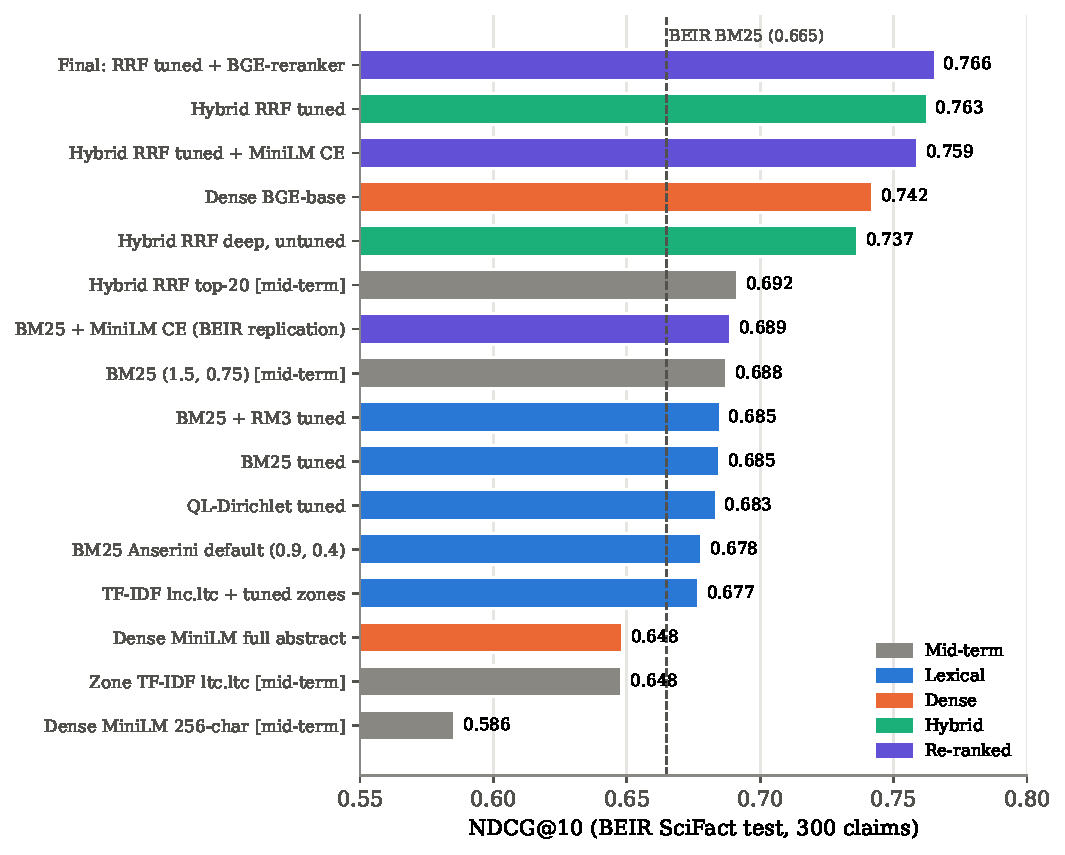
\includegraphics[width=\columnwidth]{figures/fig_retrieval_ndcg.pdf}
\caption{NDCG@10 of all systems on SciFact test; the dashed line is BM25 as reported in BEIR \cite{thakur2021beir}.}
\label{fig:ndcg}
\end{figure}

Table~\ref{tab:retrieval} and Fig.~\ref{fig:ndcg} show the results and Table~\ref{tab:steps} isolates each step. Correcting
the TF-IDF weighting to lnc.ltc gains $+0.029$ NDCG@10. Lexical tuning, query likelihood and RM3 all stay within about
$0.01$ of the mid-term BM25 (no significant differences): on SciFact, lexical matching saturates near $0.68$--$0.69$.
Encoding full abstracts instead of 256 characters gains $+0.063$ for MiniLM, and BGE adds $+0.094$. Tuned fusion adds a
further, significant $+0.021$ over BGE alone; the tuned weights give BM25 weight 0 because TF-IDF and QL already carry the
lexical signal, confirming that the mid-term fusion counted correlated lexical evidence twice. Cross-encoder re-ranking
adds only $+0.003$ (not significant) once fusion is strong. Train and test NDCG@10 of the tuned fusion are close (0.781
vs.\ 0.763), indicating no overfitting. Overall the final system improves NDCG@10 from 0.688/0.692 (mid-term BM25/hybrid)
to \textbf{0.766} and R@10 from 0.825 to 0.897. Because most claims have about one relevant abstract, P@10 is bounded near
0.1 and should not be read as low precision.

\textbf{Comparison with the BEIR paper.} Table~\ref{tab:beir} compares with SciFact results reported by Thakur et
al.\ \cite{thakur2021beir}. Our from-scratch BM25 (0.678) and our replication of their BM25+CE re-ranking (0.689 vs.\ 0.688)
match the paper closely, which validates the evaluation; our final system exceeds every reported system. Note that BEIR
models are zero-shot, while we tuned a handful of hyperparameters (no model weights) on SciFact train.

\begin{table}[t]
\centering
\caption{Comparison with BEIR \cite{thakur2021beir} on SciFact (NDCG@10)}
\label{tab:beir}
\footnotesize
\setlength{\tabcolsep}{2.5pt}
\begin{tabular}{@{}lc|lc@{}}
\toprule
BEIR paper & NDCG@10 & This work & NDCG@10 \\
\midrule
BM25 & 0.665 & BM25 (Anserini def.) & 0.678 \\
DPR / ANCE & 0.318 / 0.507 & BM25 + CE (replication) & 0.689 \\
TAS-B / GenQ & 0.643 / 0.644 & BGE-base & 0.742 \\
ColBERT / docT5q. & 0.671 / 0.675 & RRF tuned & 0.763 \\
BM25+CE (best) & 0.688 & \textbf{Final pipeline} & \textbf{0.766} \\
\bottomrule
\end{tabular}
\end{table}

\subsection{Generation}
\begin{table}[t]
\centering
\caption{LLM verdict generation (300 test claims) with different evidence}
\label{tab:gen}
\footnotesize
\begin{tabular}{@{}lccc@{}}
\toprule
Evidence given to the LLM & Evid.\ R@5 & Accuracy & Macro-F1 \\
\midrule
Mid-term hybrid, top-5 & 0.817 & 0.557 & 0.417 \\
Final retriever, top-5 & 0.840 & 0.553 & 0.414 \\
Oracle (gold cited abstracts) & 1.000 & 0.627 & 0.469 \\
\bottomrule
\end{tabular}
\end{table}
The LLM followed the output format in 100\% of cases, produced 2.2 sentences per answer, and cited an abstract outside its
context in only 0.15\% of sentences. Table~\ref{tab:gen} shows two weaknesses. First, the LLM \textbf{never predicted
REFUTED}: of 64 contradicted claims, 48 became NEI and 16 SUPPORT. Second, better retrieval did not improve verdicts: the
final retriever adds only 2.3 points of evidence recall in the top-5, and even oracle evidence raises accuracy by only 7
points. The bottleneck is the generator's reasoning, which motivates an independent verifier.

\subsection{Hallucination detection}\label{sec:det}
\textbf{Benchmark.} Each item is a sentence to verify against five abstracts (the claim's cited abstracts plus top
retrieved ones). \emph{Grounded} items are SciFact SUPPORT claims and human-marked rationale sentences;
\emph{hallucinated} items are CONTRADICT and NEI claims and rule-based perturbations of SUPPORT claims (polarity flips such
as \emph{increases}$\to$\emph{decreases} or \emph{is}$\to$\emph{is not}, changed numbers, swapped entities) plus sentences
from unrelated abstracts. Train: 1,819 items (896 grounded), test: 677 items (333 grounded).

\textbf{Tuning (train).} The large NLI model (\texttt{DeBERTa-v3-large-mnli-fever-anli-ling-wanli}) outperformed the base
model (train ROC-AUC 0.953 vs.\ 0.936); the best weights were $\alpha=0.75$, $\lambda=0.25$ (Fig.~\ref{fig:alpha}),
$\tau=0.641$, $\tau_h=0.660$, $\tau_l=0.561$, $\tau_c=0.96$. Adding the contradiction signal to \emph{every} sentence
lowered train F1 (0.910$\to$0.890), whereas gating it on the absence of entailment kept 0.910, so the latter rule was used.

\begin{table}[t]
\centering
\caption{Hallucination detection on the test benchmark (677 sentences; positive = hallucinated; thresholds from train)}
\label{tab:det}
\footnotesize
\setlength{\tabcolsep}{3.5pt}
\begin{tabular}{@{}lcccccc@{}}
\toprule
Detector & AUC & PR-AUC & P & R & F1 & Acc \\
\midrule
RTS v1 (mid-term) & 0.660 & 0.688 & 0.547 & 0.872 & 0.673 & 0.569 \\
SBERT span similarity & 0.884 & 0.870 & 0.735 & \best{1.000} & 0.847 & 0.817 \\
NLI only (max $P_e$) & 0.933 & 0.904 & 0.854 & 0.968 & 0.907 & 0.900 \\
\textbf{RTS v2} & \best{0.958} & \best{0.950} & \best{0.864} & 0.956 & \best{0.908} & \best{0.901} \\
RTS v2 with base NLI & 0.933 & -- & -- & -- & 0.885 & -- \\
\bottomrule
\end{tabular}
\end{table}

\begin{table}[t]
\centering
\caption{\% of test sentences flagged as hallucinated, by category (higher is better for hallucinated rows)}
\label{tab:cat}
\footnotesize
\setlength{\tabcolsep}{3pt}
\begin{tabular}{@{}lrcccc@{}}
\toprule
Category (truth) & $n$ & RTS v1 & SBERT & NLI & RTS v2 \\
\midrule
claim CONTRADICT (hall.) & 64 & 82.8 & 100 & 98.4 & 96.9 \\
claim NEI (hall.) & 112 & 92.0 & 100 & 95.5 & 94.6 \\
perturbed: negation (hall.) & 90 & 75.6 & 100 & 95.6 & 95.6 \\
perturbed: number (hall.) & 7 & 71.4 & 100 & 100 & 100 \\
perturbed: entity (hall.) & 27 & 100 & 100 & 96.3 & 88.9 \\
unrelated sentence (hall.) & 44 & 100 & 100 & 100 & 100 \\
\midrule
claim SUPPORT (grounded) & 124 & 79.0 & 100 & 46.0 & 41.9 \\
rationale sentence (grounded) & 209 & 71.8 & 0.0 & 0.0 & 0.0 \\
\bottomrule
\end{tabular}
\end{table}

\begin{figure*}[t]
\centering
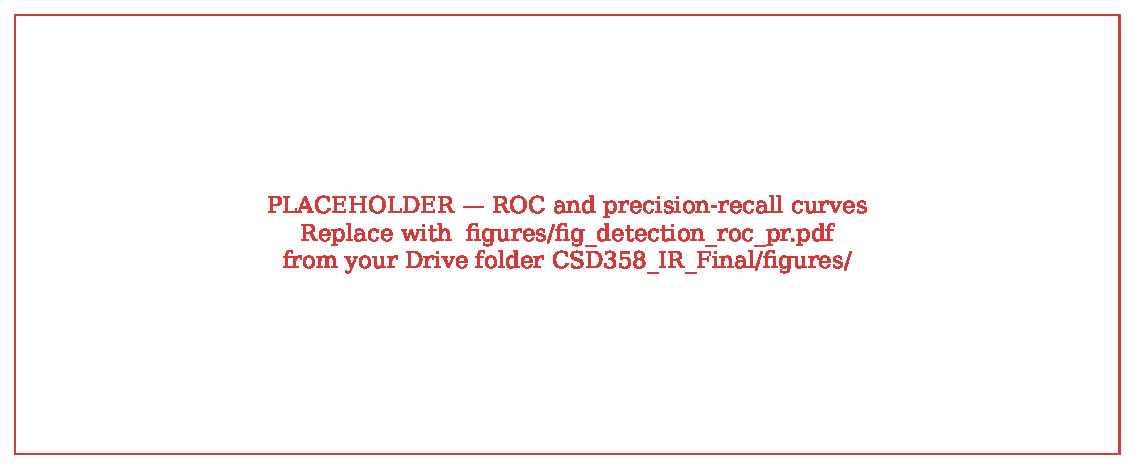
\includegraphics[width=0.82\textwidth]{figures/fig_detection_roc_pr.pdf}
\caption{ROC (left) and precision--recall (right) curves for hallucination detection on the test benchmark.}
\label{fig:roc}
\end{figure*}

\begin{figure}[t]
\centering
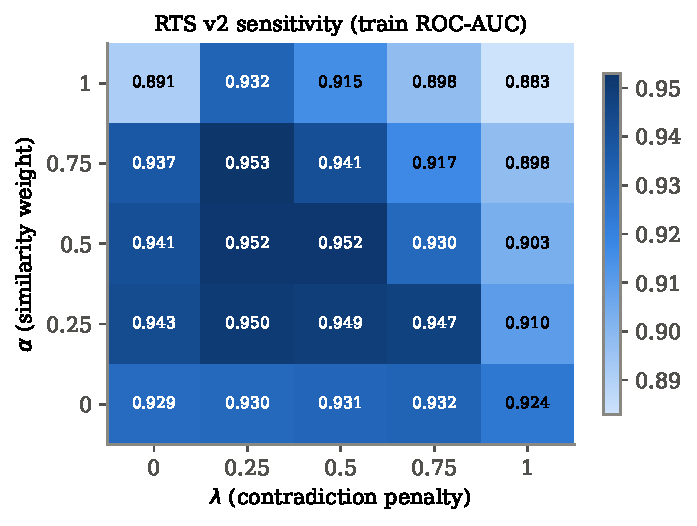
\includegraphics[width=0.85\columnwidth]{figures/fig_rts_alpha_lambda.pdf}
\caption{Sensitivity of RTS v2 to $\alpha$ and $\lambda$ (train ROC-AUC). Both pure similarity ($\alpha=1$) and pure NLI
($\alpha=0$) are worse than the combination; a moderate contradiction penalty helps.}
\label{fig:alpha}
\end{figure}

\textbf{Test results.} Table~\ref{tab:det}, Table~\ref{tab:cat} and Fig.~\ref{fig:roc} show that RTS~v2 is the best
detector on every threshold-free metric and on precision, F1 and accuracy. Against RTS~v1 it is right in 237 cases where
v1 is wrong and wrong in only 12 (exact McNemar $p=2.1\times10^{-55}$; $\Delta$F1 $=+0.235$, 95\% CI $[0.203, 0.267]$).
RTS~v1 misses one in four negations and flags 72\% of true rationale sentences; SBERT similarity effectively measures
\emph{verbatim copying}: it flags every paraphrased true claim and no copied sentence. Compared with NLI only, F1 is tied
(0.908 vs.\ 0.907), but RTS~v2 ranks sentences better (ROC-AUC $+0.025$, PR-AUC $+0.046$), which is what a transparency
score needs. The main error is on human-paraphrased SUPPORT claims (42\% flagged), where NLI fails to recognise
entailment of generalised wording.

\textbf{Human evaluation on real LLM output.} We labelled 80 randomly sampled factual sentences from the LLM's test answers
(blind to RTS scores) as grounded (45), unsupported (29) or contradicted (6). Table~\ref{tab:human} shows that RTS~v2 is
again the best detector (highest ROC-AUC, precision and accuracy), and that RTS~v1 is \emph{worse than random} (AUC 0.37):
unsupported LLM sentences reuse the abstracts' wording and then add an unsupported inference, so they look similar.
However, all detectors are far weaker than on the benchmark (RTS~v2 AUC 0.573 vs.\ 0.958). Most real errors are subtle
\emph{unsupported} statements (over-generalisations, partially supported sentences, invented conclusions) rather than
contradictions, and sentence-level NLI handles them poorly; 11 of 31 sentences labelled HIGH were judged unsupported. With
$n=80$ and one annotator (standard error of AUC $\approx0.06$), only the gap to RTS~v1 is clearly meaningful.

\begin{table}[t]
\centering
\caption{Detection vs.\ human labels on 80 real LLM sentences (positive = not grounded)}
\label{tab:human}
\footnotesize
\setlength{\tabcolsep}{3.5pt}
\begin{tabular}{@{}lccccc@{}}
\toprule
Detector & AUC & P & R & F1 & Acc \\
\midrule
RTS v1 (mid-term) & 0.370 & 0.353 & 0.514 & 0.419 & 0.375 \\
SBERT span similarity & 0.495 & 0.443 & \best{1.000} & \best{0.614} & 0.450 \\
NLI only & 0.540 & 0.510 & 0.743 & 0.605 & 0.575 \\
\textbf{RTS v2} & \best{0.573} & \best{0.524} & 0.629 & 0.571 & \best{0.588} \\
\bottomrule
\end{tabular}
\end{table}

\subsection{Claim verification and comparison with SciFact}
\begin{table}[t]
\centering
\caption{Claim verification on 300 test claims (final retriever's evidence unless noted)}
\label{tab:verif}
\footnotesize
\setlength{\tabcolsep}{3pt}
\begin{tabular}{@{}lccccc@{}}
\toprule
System & Acc & Macro-F1 & F1$_{S}$ & F1$_{C}$ & F1$_{N}$ \\
\midrule
LLM only & 0.553 & 0.414 & 0.667 & 0.000 & 0.576 \\
NLI only & 0.667 & 0.664 & 0.673 & 0.644 & 0.675 \\
\textbf{LLM + RTS v2} & \best{0.677} & \best{0.673} & \best{0.709} & \best{0.644} & 0.667 \\
\midrule
LLM + RTS v2, mid-term evidence & 0.673 & 0.666 & 0.727 & 0.607 & 0.664 \\
LLM + RTS v2, oracle evidence & 0.777 & 0.770 & 0.809 & 0.723 & 0.778 \\
\bottomrule
\end{tabular}
\end{table}

\begin{figure*}[t]
\centering
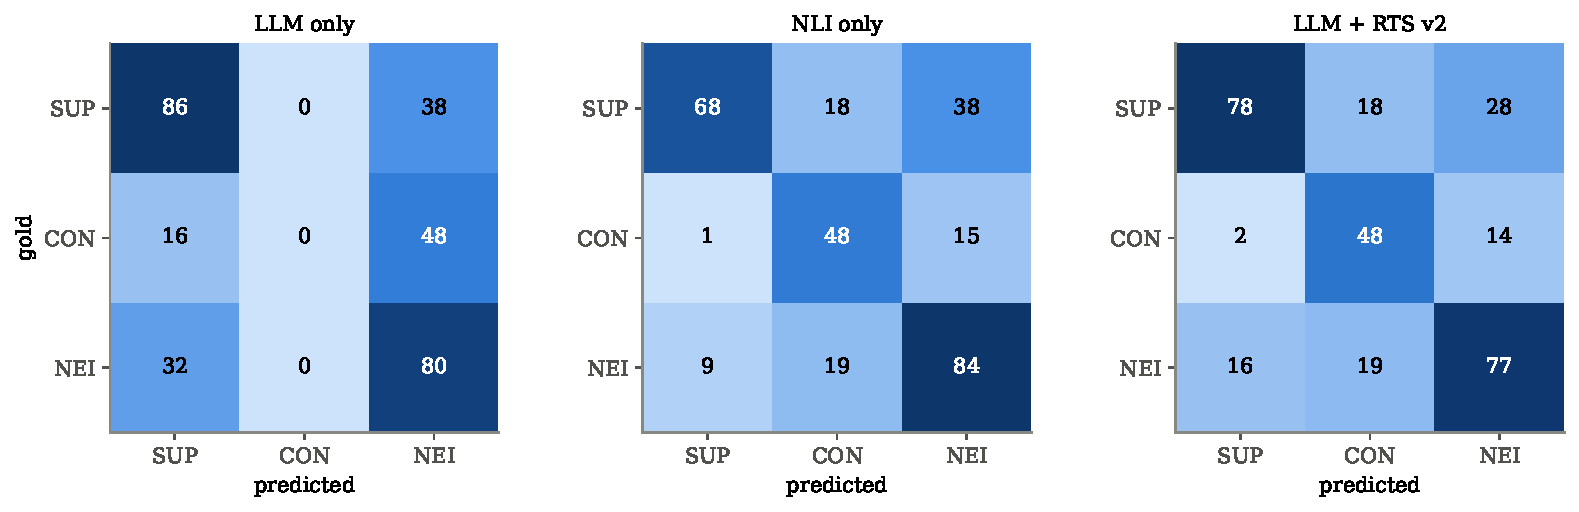
\includegraphics[width=0.78\textwidth]{figures/fig_verdict_confusion.pdf}
\caption{Confusion matrices of the three verdict systems on the test claims (rows: gold; columns: predicted).}
\label{fig:cm}
\end{figure*}

The verdict thresholds tuned on 200 train claims were $\theta_c=0.95$, $\theta_e=0.70$, $\theta_r=0.60$.
Table~\ref{tab:verif} and Fig.~\ref{fig:cm} show that RTS-guided correction raises accuracy from 0.553 to 0.677 and
macro-F1 from 0.414 to 0.673, mainly by detecting refuted claims (CONTRADICT F1 0.00$\to$0.64). The claim-level NLI check
provides most of the gain; the hybrid adds a small improvement over NLI alone, while the LLM contributes the readable,
cited explanation.

\textbf{Comparison with Wadden et al.\ \cite{wadden2020scifact}.} We apply the SciFact abstract-level
\emph{label-only} protocol: a predicted (claim, abstract, label) is correct if the abstract is a gold evidence abstract
and the label matches; precision and recall are micro-averaged, with at most three abstracts per claim. Since our test set is
SciFact's dev set, we compare with the paper's dev results (Table~\ref{tab:scifact}). In the open (retrieval) setting our
system reaches F1 56.6 versus 51.0 for VeriSci, mainly through recall (57.4 vs.\ 47.5). With oracle abstracts it is 2
points below VeriSci, which is a RoBERTa-large model trained on SciFact, whereas our verifier uses an off-the-shelf NLI
model and only tunes thresholds; our oracle context is also harder because it includes non-evidence abstracts.

\begin{table}[t]
\centering
\caption{Abstract-level label-only results on SciFact dev (= our test), compared with Wadden et al.\ \cite{wadden2020scifact}}
\label{tab:scifact}
\footnotesize
\setlength{\tabcolsep}{3pt}
\begin{tabular}{@{}llccc@{}}
\toprule
Setting & System & P & R & F1 \\
\midrule
\multirow{4}{*}{Open} & VeriSci \cite{wadden2020scifact} & 55.4 & 47.5 & 51.0 \\
& Zero-shot \cite{wadden2020scifact} & 52.7 & 41.6 & 46.5 \\
& Ours: NLI only & \best{56.9} & 53.6 & 55.2 \\
& \textbf{Ours: LLM + RTS v2} & 55.8 & \best{57.4} & \best{56.6} \\
\midrule
\multirow{3}{*}{Oracle} & VeriSci \cite{wadden2020scifact} & \best{91.0} & 67.4 & \best{77.4} \\
& Zero-shot \cite{wadden2020scifact} & 88.9 & 58.3 & 70.4 \\
& \textbf{Ours: LLM + RTS v2} & 79.4 & \best{71.8} & 75.4 \\
\bottomrule
\end{tabular}
\end{table}

\subsection{Selective answering}
\begin{figure}[t]
\centering
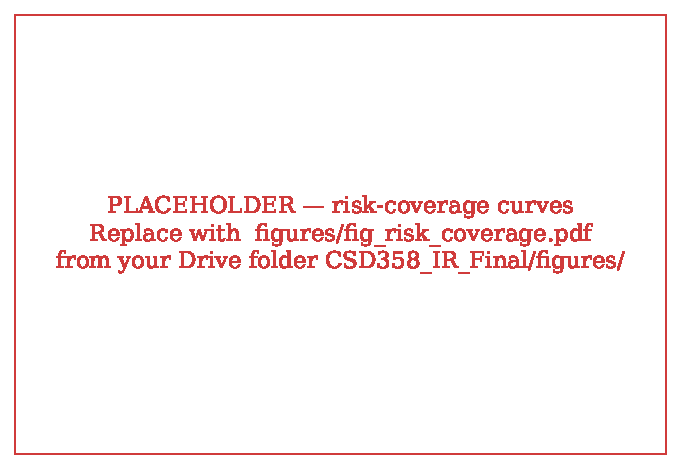
\includegraphics[width=0.95\columnwidth]{figures/fig_risk_coverage.pdf}
\caption{Verdict accuracy when only the most confident claims are answered (test).}
\label{fig:rc}
\end{figure}
We ranked claims by confidence and answered only the top fraction (Fig.~\ref{fig:rc}). Claim-level NLI confidence
$\max(E,C)$ is useful: accuracy rises from 0.68 at full coverage to 0.76 at 25\% coverage (AURC 0.294). The answer-level
$\RTS_{\min}$, however, is no better than random (AURC 0.335 vs.\ 0.323). This negative result shows that
\emph{faithfulness is not correctness}: an explanation can be well grounded while its verdict is wrong. Answers that
consist only of abstentions have no RTS, which further limits this use.

\subsection{Generalisation to unseen collections}
\begin{table}[t]
\centering
\caption{Zero-shot generalisation (NDCG@10), no re-tuning}
\label{tab:gen2}
\footnotesize
\setlength{\tabcolsep}{3pt}
\begin{tabular}{@{}lccc@{}}
\toprule
System & SciFact & NFCorpus & FiQA \\
\midrule
BM25 as reported in BEIR \cite{thakur2021beir} & 0.665 & 0.325 & 0.236 \\
Our BM25 (Anserini defaults) & 0.678 & 0.326 & 0.240 \\
BGE-base & 0.742 & 0.371 & 0.405 \\
RRF (SciFact-tuned weights) & 0.763 & 0.380 & 0.424 \\
\textbf{Final pipeline} & \best{0.766} & \best{0.383} & \best{0.432} \\
\bottomrule
\end{tabular}
\end{table}
Table~\ref{tab:gen2} applies the frozen pipeline to NFCorpus (medical, 3.6K documents) and FiQA (finance, 57.6K documents).
Our BM25 reproduces BEIR's numbers on both, and the ordering BM25 $<$ BGE $<$ hybrid $<$ final holds on all three
collections; on FiQA the final pipeline improves NDCG@10 by $0.19$ over BM25 on an 11$\times$ larger, out-of-domain
corpus. Most of the zero-shot gain comes from BGE, whose large training data may overlap in domain with these benchmarks.

\subsection{Discussion}
The retrieval objective (O1) is met with significant, step-wise gains and strong external validity. Generation (O2) is
reliable in format and citation validity but weak in reasoning. RTS~v2 (O3) clearly improves on RTS~v1 and on its own
components on human-labelled claims and controlled perturbations, and makes every decision inspectable through the evidence
span, entailment probabilities and citation check. It markedly improves verdicts (O4), and it compares favourably with
published systems (O5). The human evaluation shows, however, that detecting subtle unsupported statements in real LLM text
remains hard, and that benchmark results overestimate real-world performance.

% =====================================================================
% 9. CONCLUSIONS AND LIMITATIONS
% =====================================================================
\section{Conclusions and Limitations}
We extended a mid-term hybrid RAG prototype into a complete, rigorously evaluated system for transparent scientific claim
verification. A tuned hybrid of from-scratch lexical models, dense encoders, weighted RRF and re-ranking reaches NDCG@10
0.766 on SciFact and generalises to two unseen collections. RTS~v2 combines span attribution, similarity, NLI, a
contradiction penalty and citation checks into an interpretable per-sentence trust score that detects hallucinated
sentences far better than similarity alone (ROC-AUC 0.958 vs.\ 0.660) and turns a generator that never refutes into a
verifier with macro-F1 0.673, outperforming the SciFact VeriSci baseline in the open setting.

\textbf{Limitations.} (1) On real LLM sentences detection is much weaker (ROC-AUC 0.573) than on the benchmark; subtle
unsupported statements dominate real errors. (2) The human evaluation uses 80 sentences and a single annotator. (3) NLI
misses entailment for paraphrased or generalised claims (42\% of true SUPPORT claims flagged). (4) Perturbations are
rule-based and simpler than real hallucinations. (5) A 3B-parameter LLM was used because of the T4 GPU; larger models may
reason better. (6) Re-ranking gave no significant gain, and part of the zero-shot gains comes from BGE's pre-training.
(7) Answer-level RTS does not predict verdict correctness, and abstention-only answers receive no score. (8) Only English
abstracts were studied.

\textbf{Future work.} Decomposing sentences into atomic facts before verification \cite{min2023factscore}, biomedical or
SciFact-trained NLI models, calibrating thresholds on real generated text, and larger generators.

% =====================================================================
% 10. REFERENCES
% =====================================================================
\begin{thebibliography}{99}
\footnotesize

\bibitem{lewis2020rag}
Lewis, P., Perez, E., Piktus, A., Petroni, F., Karpukhin, V., Goyal, N., K\"uttler, H., Lewis, M., Yih, W.T.,
Rockt\"aschel, T., Riedel, S. and Kiela, D., 2020, December. Retrieval-augmented generation for knowledge-intensive NLP
tasks. In Advances in Neural Information Processing Systems 33 (pp. 9459--9474).

\bibitem{thakur2021beir}
Thakur, N., Reimers, N., R\"uckl\'e, A., Srivastava, A. and Gurevych, I., 2021, December. BEIR: A heterogeneous benchmark
for zero-shot evaluation of information retrieval models. In Proceedings of the Neural Information Processing Systems
Track on Datasets and Benchmarks 1.

\bibitem{wadden2020scifact}
Wadden, D., Lin, S., Lo, K., Wang, L.L., van Zuylen, M., Cohan, A. and Hajishirzi, H., 2020, November. Fact or fiction:
Verifying scientific claims. In Proceedings of the 2020 Conference on Empirical Methods in Natural Language Processing
(pp. 7534--7550).

\bibitem{robertson2009bm25}
Robertson, S. and Zaragoza, H., 2009. The probabilistic relevance framework: BM25 and beyond. Foundations and Trends in
Information Retrieval, 3(4), pp. 333--389.

\bibitem{zhai2001smoothing}
Zhai, C. and Lafferty, J., 2001, September. A study of smoothing methods for language models applied to ad hoc information
retrieval. In Proceedings of the 24th Annual International ACM SIGIR Conference on Research and Development in
Information Retrieval (pp. 334--342).

\bibitem{lavrenko2001relevance}
Lavrenko, V. and Croft, W.B., 2001, September. Relevance-based language models. In Proceedings of the 24th Annual
International ACM SIGIR Conference on Research and Development in Information Retrieval (pp. 120--127).

\bibitem{cormack2009rrf}
Cormack, G.V., Clarke, C.L.A. and B\"uttcher, S., 2009, July. Reciprocal rank fusion outperforms Condorcet and individual
rank learning methods. In Proceedings of the 32nd International ACM SIGIR Conference on Research and Development in
Information Retrieval (pp. 758--759).

\bibitem{manning2008ir}
Manning, C.D., Raghavan, P. and Sch\"utze, H., 2008. Introduction to Information Retrieval. Cambridge University Press.

\bibitem{reimers2019sbert}
Reimers, N. and Gurevych, I., 2019, November. Sentence-BERT: Sentence embeddings using Siamese BERT-networks. In
Proceedings of the 2019 Conference on Empirical Methods in Natural Language Processing and the 9th International Joint
Conference on Natural Language Processing (pp. 3982--3992).

\bibitem{xiao2024cpack}
Xiao, S., Liu, Z., Zhang, P., Muennighoff, N., Lian, D. and Nie, J.Y., 2024, July. C-Pack: Packed resources for general
Chinese embeddings. In Proceedings of the 47th International ACM SIGIR Conference on Research and Development in
Information Retrieval (pp. 641--649).

\bibitem{johnson2021faiss}
Johnson, J., Douze, M. and J\'egou, H., 2021. Billion-scale similarity search with GPUs. IEEE Transactions on Big Data,
7(3), pp. 535--547.

\bibitem{nogueira2019passage}
Nogueira, R. and Cho, K., 2019. Passage re-ranking with BERT. arXiv preprint arXiv:1901.04085.

\bibitem{gao2023alce}
Gao, T., Yen, H., Yu, J. and Chen, D., 2023, December. Enabling large language models to generate text with citations. In
Proceedings of the 2023 Conference on Empirical Methods in Natural Language Processing (pp. 6465--6488).

\bibitem{thorne2018fever}
Thorne, J., Vlachos, A., Christodoulopoulos, C. and Mittal, A., 2018, June. FEVER: a large-scale dataset for fact
extraction and VERification. In Proceedings of the 2018 Conference of the North American Chapter of the Association for
Computational Linguistics: Human Language Technologies (pp. 809--819).

\bibitem{ji2023survey}
Ji, Z., Lee, N., Frieske, R., Yu, T., Su, D., Xu, Y., Ishii, E., Bang, Y.J., Madotto, A. and Fung, P., 2023. Survey of
hallucination in natural language generation. ACM Computing Surveys, 55(12), pp. 1--38.

\bibitem{honovich2022true}
Honovich, O., Aharoni, R., Herzig, J., Taitelbaum, H., Kukliansy, D., Cohen, V., Scialom, T., Szpektor, I., Hassidim, A.
and Matias, Y., 2022, July. TRUE: Re-evaluating factual consistency evaluation. In Proceedings of the 2022 Conference of
the North American Chapter of the Association for Computational Linguistics: Human Language Technologies (pp. 3905--3920).

\bibitem{laban2022summac}
Laban, P., Schnabel, T., Bennett, P.N. and Hearst, M.A., 2022. SummaC: Re-visiting NLI-based models for inconsistency
detection in summarization. Transactions of the Association for Computational Linguistics, 10, pp. 163--177.

\bibitem{he2023debertav3}
He, P., Gao, J. and Chen, W., 2023, May. DeBERTaV3: Improving DeBERTa using ELECTRA-style pre-training with
gradient-disentangled embedding sharing. In Proceedings of the Eleventh International Conference on Learning
Representations.

\bibitem{manakul2023selfcheckgpt}
Manakul, P., Liusie, A. and Gales, M., 2023, December. SelfCheckGPT: Zero-resource black-box hallucination detection for
generative large language models. In Proceedings of the 2023 Conference on Empirical Methods in Natural Language
Processing (pp. 9004--9017).

\bibitem{min2023factscore}
Min, S., Krishna, K., Lyu, X., Lewis, M., Yih, W.T., Koh, P.W., Iyyer, M., Zettlemoyer, L. and Hajishirzi, H., 2023,
December. FActScore: Fine-grained atomic evaluation of factual precision in long form text generation. In Proceedings of
the 2023 Conference on Empirical Methods in Natural Language Processing (pp. 12076--12100).

\bibitem{qwen2024}
Yang, A., Yang, B., Zhang, B., Hui, B., Zheng, B., Yu, B., Li, C., Liu, D., Huang, F., Wei, H. et al., 2024. Qwen2.5
technical report. arXiv preprint arXiv:2412.15115.

\end{thebibliography}

\end{document}
